\documentclass[10pt]{ujarticle}
\usepackage{float}
\usepackage{adrobo_abst}
\usepackage{graphicx}
\usepackage[dvipdfmx]{color}
\usepackage{amssymb,amsmath}
\usepackage{bm}
\usepackage[superscript]{cite}
\usepackage{enumerate}
\usepackage{url}
% \usepackage[dvipdfmx]{color}
%\usepackage[absolute]{textpos}

\renewcommand\citeform[1]{(#1)}

\begin{document}
    
    \makeatletter
    \doctype{2022年度卒業論文概要}
    \title{視覚と行動のend-to-end学習により\\経路追従行動をオンラインで模倣する手法の提案}{(オフラインでデータセットを収集して訓練する手法の提案)}
    \etitle{A proposal for an online imitation method of path-tracking behavior by end-to-end learning of vision and action}{(Validation of a method to collect and train dataset offline)}
    
    \author{19C1068\hspace{.5zw}髙橋祐樹}
    \eauthor{Yuuki TAKAHASHI}
    
    \makeatother
    
    \abstract{In this paper, we propose an off-line data collection and training method based on the method proposed by Okada et al. to imitate path-following behavior. In the proposed method, the robot is placed on and around the target path and collects data for offline training. Experimental results show the effectiveness of the proposed method.}
    
    \keywords{End-to-End Learning, Navigation, Offline}
    
    \maketitle
    
    \supervisor{指導教員:林原靖男 教授}
    
    \section{緒\hspace{2zw}言}%===========================
    近年, 自律移動ロボットの研究が盛んに行われている. Bojarskiら\cite{bojarski}は人が操作するステアリングの角度をend-to-end学習することで, 自律走行する手法を提案した. また, 岡田ら\cite{si2020-okada}(以下「従来研究」と称する)は2D-LiDARを用いた自律移動システムの出力を学習させることで, 経路追従行動をオンラインで模倣する手法を提案し, 実験によりその有効性を確認してきた. 本研究では, 従来研究を基に目標経路上及び周辺のデータを一度に収集し, オフラインで訓練する手法を提案する. 訓練後は, カメラ画像を入力とした学習器の出力で自律走行させることで手法の有効性を検証する. 
    % しかし, カメラ画像を入力とした学習器の出力で自律走行をするには, ロボットを何周も走行させて学習する必要があり, 手間や時間が掛かる.
    % また, 清岡ら\cite{si2021-kiyooka}により, 経路上だけでなく経路から離れた状態も学習することが, 経路追従行動を模倣する上で有効であることも示されている.
    
    \section{従来手法}%===========================
    従来研究では, 地図を用いたルールベース制御器の出力を模倣し, 視覚に基づく経路追従行動を獲得した. 図\ref{Fig:si2020-okada}に示すシステムでは, LiDAR, オドメトリを入力としたナビゲーションの出力である角速度を学習器とモータ駆動系に与える. ナビゲーションの角速度は, ROSのパッケージであるnavigation\cite{navigation}により計算される. また, 学習器には, カメラ画像を64×48にリサイズした3つのカメラ画像(RGB画像)を入力し, ナビゲーションの角速度を出力してend-to-end学習する. 左右のカメラ画像に対する角速度には, それぞれ経路に戻るようなオフセットを加える. 学習後は, カメラ画像を入力とした学習器の出力により走行する. 

    \begin{figure}[h]
        \centering
        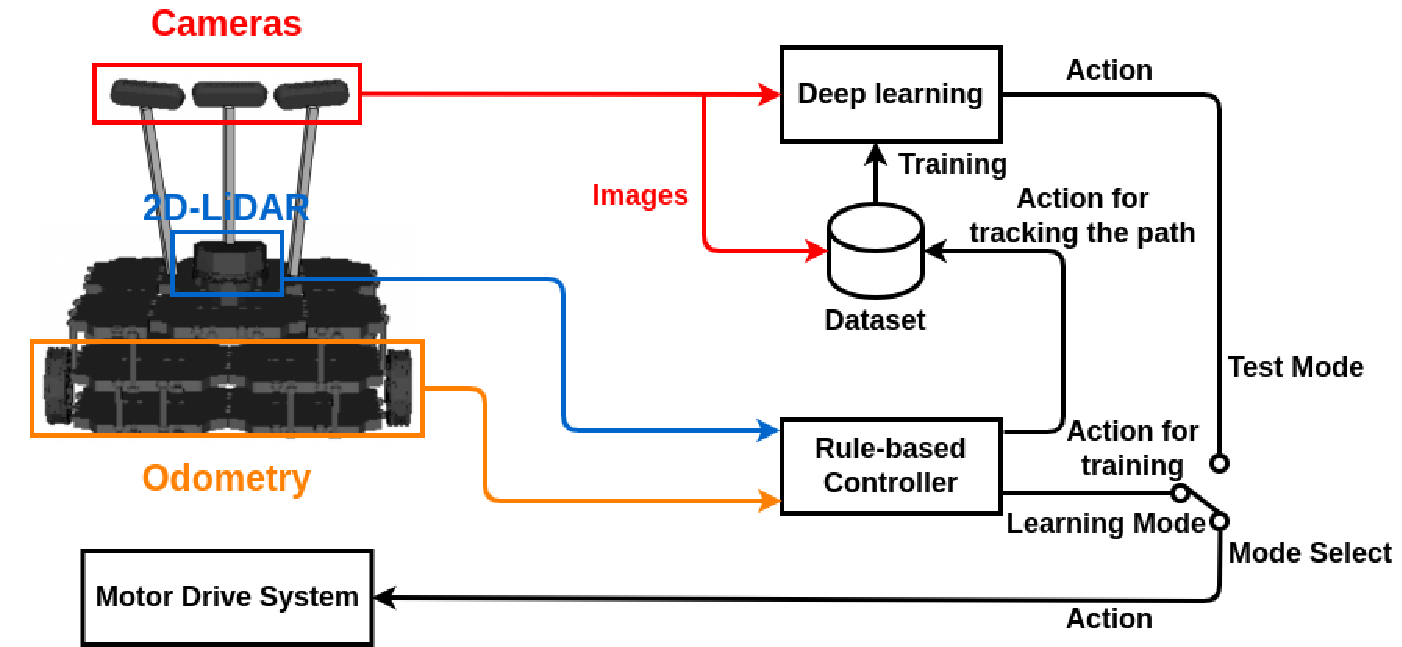
\includegraphics[keepaspectratio, scale=0.3]{fig/okada.pdf}
        \caption{Systems that imitation learning for map-based navigation from\cite{si2020-okada}}
        \label{Fig:si2020-okada}
    \end{figure}

    \section{提案手法}%===========================
    次に, 従来研究を基にしたオフラインでデータを収集し訓練するする手法を提案する. 図\ref{Fig:collect}にデータの収集方法を示す. ロボットを赤線の目標経路から平行に離れた座標に配置して, その座標ごとに経路に沿った向きを基準に傾けて, カメラ画像とナビゲーションの出力である角速度を図\ref{Fig:collect}のように収集する. このように, ロボットを走行させることなく, 配置することで, 一度に大量のデータを収集することができる. その後, 収集したデータを用いてオフラインで学習を行う. 

    \begin{figure}[h]
        \centering
        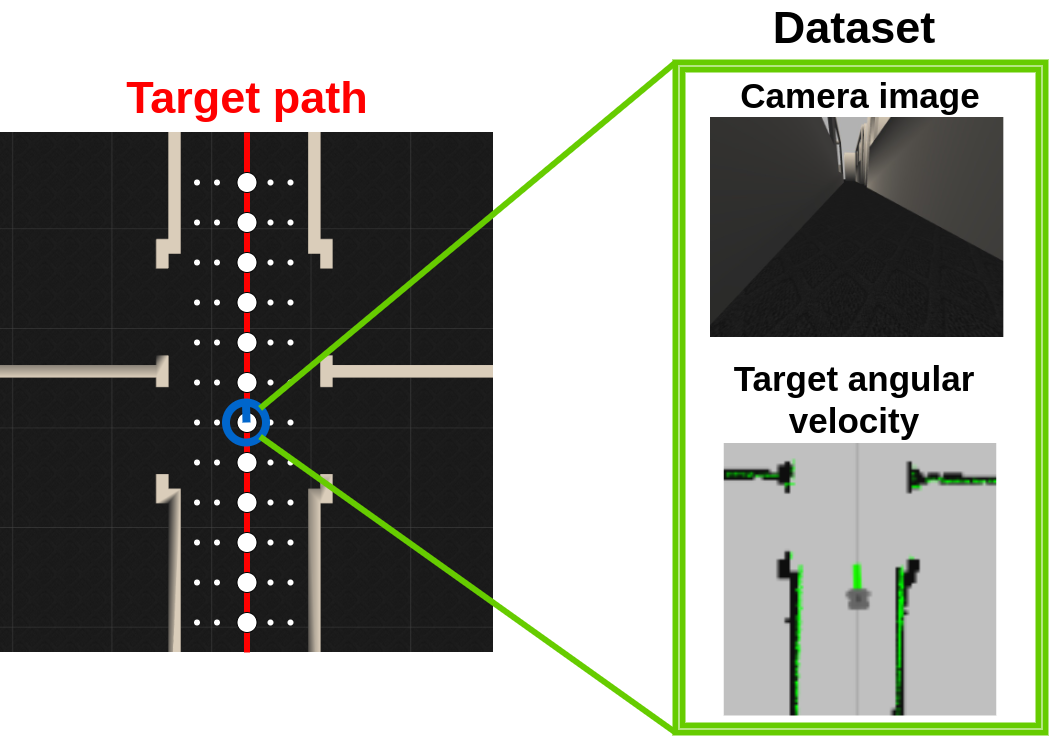
\includegraphics[width=0.3\textwidth]{fig/collect-data2.png}
        \caption{Method of collecting data around the target route}
        \label{Fig:collect}
    \end{figure}

    \section{シミュレータを用いた実験}%=========================== 
    \subsection{実験装置}\mbox{}\\
    シミュレータにはGazeboのWillow Garage\cite{willow}を用いて, 図\ref{Fig:willow}に示すコースで一周行う. また, ロボットモデルにはカメラを3つ搭載したTurtlebo3\cite{turtlebot3}を用いた. 

    \begin{figure}[h]
        \centering
        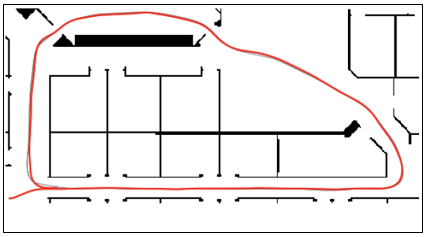
\includegraphics[width=0.3\textwidth]{fig/willow-garage.png}
        \caption{Course to collect data}
        \label{Fig:willow}
    \end{figure}

    \subsection{実験方法}
    \begin{enumerate}
        \item{データ収集フェーズ}\mbox{}\\図\ref{Fig:collect-data}にデータの収集方法を示す. 赤線の目標経路から平行に±0.01, ±0.02, ±0.04, ±0.06, ±0.08, ±0.10, ±0.15, ±0.20, ±0.30[m]離れた座標にロボットを配置する. そして, その座標ごとに経路に沿った向きを基準として±5度傾けて, カメラ画像とナビゲーションの出力である角速度を収集する. 
        \item{訓練フェーズ}\mbox{}\\データ量及びバッチサイズ7242, バッチ学習で4000step, 8000step, 10000step学習した. 
        % なお, 4000stepは従来研究において, シミュレータの実験に用いられてきたステップ数であり, 10000stepは従来研究において, 実ロボットの実験に用いられていたステップ数である. 
        % 従来研究ではオンラインで学習を行うため計算のリソースなどの観点からバッチサイズを8にして, 全てのデータを使用していなかった. しかし, 本研究では
        \item{テストフェーズ}\mbox{}\\図\ref{Fig:willow}に示したコースで10回走行させる. 経路を一周できた場合を成功とし, 壁に衝突したり, 目標経路から10[m]以上離れたりした場合を失敗とした. 
    \end{enumerate}

    \begin{figure}[h]
        \centering
        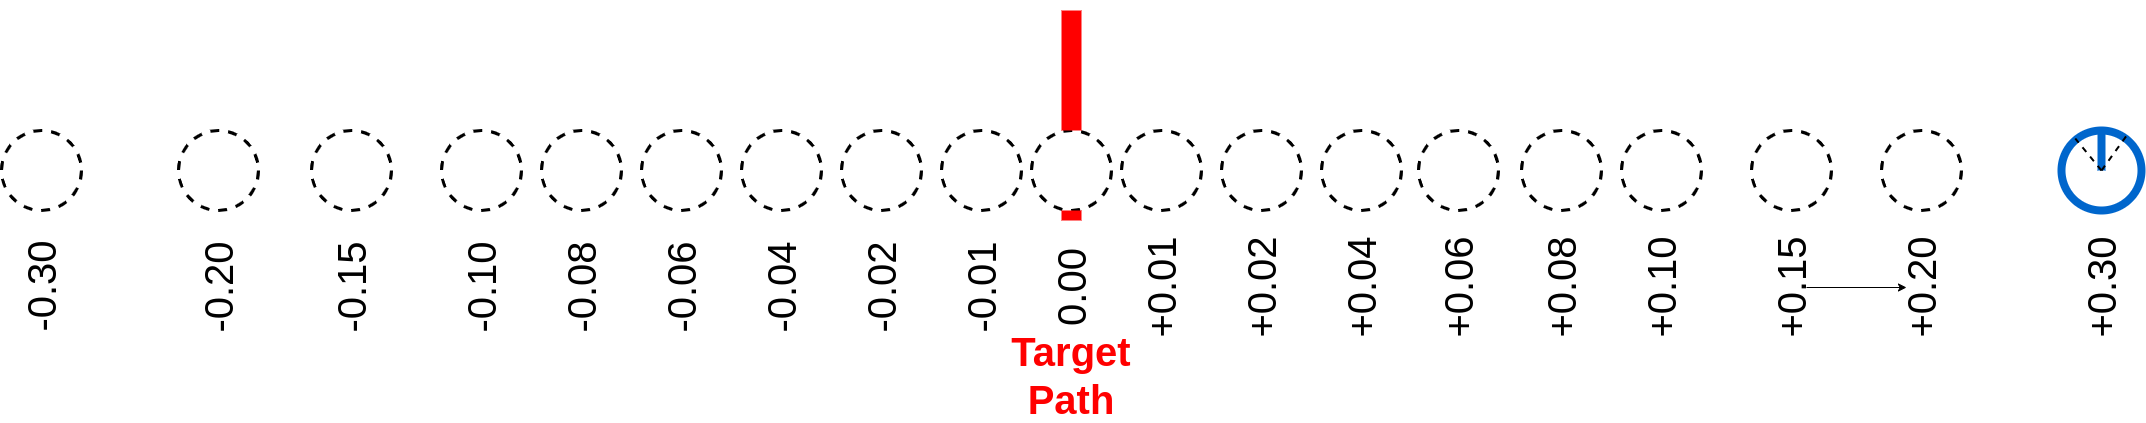
\includegraphics[width=0.45\textwidth]{fig/collect-data.png}
        \caption{Method of collecting data around the target route}
        \label{Fig:collect-data}
    \end{figure}

    \subsection{実験結果}\mbox{}\\
    実験結果を表\ref{tb:result}に示す. 4000stepでは成功回数が0だったが, 8000step, 10000stepでは成功回数が増えた. また, 図\ref{Fig:loss}からステップ数増やすことで学習が収束していることが確認できる. 従って, 訓練する際にバッチ学習を用いて, ステップ数を増やすことで成功回数が増えることを示せた. 

    \begin{table}[h]
        \centering
        \scalebox{0.7}{
        \begin{tabular}{|c|c|} \hline
          Experiments & Number of successes \\ \hline
          Exp.1(4000step) & 0/10 \\ \hline
          Exp.2(8000step) & 1/10 \\ \hline
          Exp.3(10000step) & 1/10 \\ \hline
        \end{tabular}
        }
        \caption{Number of successes in the experiment}
        \label{tb:result}
      \end{table}

    \begin{figure}[h]
        \centering
        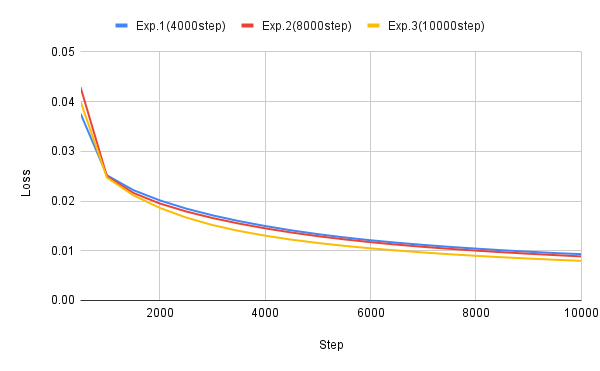
\includegraphics[width=0.35\textwidth]{fig/chart.png}
        \caption{Loss value in the experiments}
        \label{Fig:loss}
    \end{figure}

    \section{結\hspace{2zw}言}%===========================
    本稿では, 従来研究を基にオフラインでデータセットを収集して訓練する手法を提案した. そして, 実験により提案手法の有効性を確認した. 

    \vspace{5truemm}
    {\footnotesize
        \begin{thebibliography}{99}

            \bibitem{bojarski}
            Bojarsi, Mariusz, et al.:``End to End Learning for Self-Driving Cars.'', arXiv: 1604.07316, 2016
            
            \bibitem{si2020-okada}
            岡田 眞也, 清岡 優祐, 上田 隆一, 林原 靖男: ``視覚と行動のend-to-end学習により経路追従行動をオンラインで模倣する手法の提案'', \textit{計測自動制御学会 SI 部門講演会 SICE-SI2021 予稿集}, pp.1147-1152, 2020.

            % \bibitem{si2021-okada}
            % 岡田 眞也, 清岡 優祐, 春山 健太, 上田 隆一, 林原 靖男: ``視覚と行動のend-to-end学習により経路追従行動をオンラインで模倣する手法の提案-“経路追従行動の修正のためにデータセットを動的に追加する手法の検討'', \textit{計測自動制御学会 SI 部門講演会 SICE-SI2021 予稿集}, pp.1066-1070, 2021.

            % \bibitem{si2021-kiyooka}
            % 清岡 優祐, 岡田 眞也, 岩井 一輝, 上田 隆一, 林原 靖男: ``視覚と行動のend-to-end学習により経路追従行動をオンラインで模倣する手法の提案''-データセットと生成された経路追従行動の解析'', \textit{計測自動制御学会 SI 部門講演会 SICE-SI2021 予稿集}, pp.1072-1075, 2021.

            \bibitem{navigation}
            ros-planning, navigation リポジトリ\\
            \url{https://github.com/ros-planning/navigation}\\
            (最終閲覧日 \today)

            % \bibitem{gazebo}
            % gazebo リポジトリ\\
            % \url{http://gazebosim.org/}\\
            % (最終閲覧日 \today)

            \bibitem{willow}
            Koenig, Nathan, and Andrew Howard. ”design and use paradigms for gazebo, an open-source multi-robot simulator.”. 2004 IEEE/RSJ International Conference on Intelligent Robots and Systems (IROS)(IEEE Cat. No. 04CH37566). Vol. 3. IEEE, pp.2149-2154(2004).\\
            (最終閲覧日 \today)

            \bibitem{turtlebot3}
            Turtlebot3-robotis emanual.robotis.\\
            url{https://emanual.robotis.com/docs/.}\\
            (最終閲覧日 \today)
            
        \end{thebibliography}
    }
\end{document}
